\documentclass[journal]{IEEEtran}

% ---------------------------------------------------------------------------
% Cognitive Electronic Warfare in an NTTR-inspired simulated electronic
% combat range using Deep RL. Venue-neutral manuscript (IEEEtran journal class).
%
% All tables under tables/ and figures under figs/ are generated from the accepted
% five-seed JSON artifacts in results/anchors_full_ms_accepted/ by
%   uv run python              scripts/paper/extract_results_tables.py
%   uv run --with matplotlib python scripts/paper/build_figures.py
% Every numerical claim below is sourced from those files (mean +/- std over seeds).
% ---------------------------------------------------------------------------

\usepackage{cite}
\usepackage{amsmath,amssymb,amsfonts}
\usepackage{graphicx}
\usepackage{booktabs}
\usepackage{array}
\usepackage{pifont}
\usepackage{tikz}
\usetikzlibrary{arrows.meta,positioning,fit,backgrounds}
\usepackage{xcolor}
\usepackage{url}
\usepackage[hidelinks]{hyperref}

\graphicspath{{figs/}}
\newcommand{\cmark}{\textcolor{black}{\ding{51}}}
\newcommand{\xmark}{\textcolor{black}{\ding{55}}}

\begin{document}

\title{Cognitive Electronic Warfare in an NTTR-Inspired Electronic Combat Range using Deep RL:
Adaptive Jamming, Electronic Protection, and Deception Operations in a Dense Simulated Threat
Environment}

\author{Hugo Fern\'andez Sol\'is%
\thanks{H.\ Fern\'andez Sol\'is is with Projener.ai
(e-mail: hugofernandezsolis@gmail.com).}%
\thanks{Manuscript prepared 2026. All emitters, waveforms and scenario parameters used in
this work are synthetic or derived from published catalogs; no classified or operational
electronic-warfare data is used.}}

\markboth{Preprint --- Cognitive Electronic Warfare using Deep RL}%
{Fern\'andez Sol\'is: Cognitive Electronic Warfare using Deep RL}

\maketitle

\begin{abstract}
Cognitive electronic warfare (EW) replaces fixed threat-response libraries with a
sense--decide--act loop executed at machine speed, yet the literature almost always studies a
single learning component in isolation and rarely reports inference latency. We present a
cognitive EW \emph{component suite} integrated over a shared synthetic signal layer and a common
evaluation harness, exercised on an NTTR-inspired \emph{synthetic} electronic combat range; each
component is trained and evaluated independently rather than in a single closed-loop run. The
suite comprises five parts: (i) a Dueling Double DQN (D3QN) agent
for adaptive jamming, (ii) a temporal convolutional network for low-latency emitter/mode/threat
ELINT classification including low-probability-of-intercept (LPI) radars, (iii) a QMIX
multi-agent controller for coordinated EW across an aircraft formation, (iv) a Wasserstein GAN
that synthesizes radar pulse-descriptor signals for data augmentation, and (v) a deterministic
EW response library acting as a reproducible conventional baseline. Over a five-seed
full-profile GPU campaign (reporting mean $\pm$ standard deviation), the jamming agent reaches a
$1.000 \pm 0.000$ spectrum win rate (vs.\ $0.733 \pm 0.038$ for the library) at $0.53$\,ms $p99$
inference latency; the ELINT classifier attains $0.984 \pm 0.005$ macro accuracy on emitter type
and $\approx 1.000$ on mode and LPI (threat state is deterministic from mode in this catalog);
the coordinated formation improves IADS suppression
by $+259\%$ ($2.594 \pm 0.561$ relative improvement) over independent agents; and synthetic
augmentation lets the classifier recover two emitters withheld from its real training set,
raising their accuracy from $0.000$ to $0.800 \pm 0.274$ (global test accuracy
$0.657 \to 0.832$). The M1, M3, and M4 targets are met on all five seeds. The ELINT classifier meets
every accuracy target on every seed but misses its $<1$\,ms $p99$ latency target
($2.06 \pm 0.58$\,ms), which we report as a limitation. We frame the results as a
\emph{synthetic-environment} study and release the staged per-seed and aggregate artifacts,
configuration hashes and generation scripts to support reproducibility.
\end{abstract}

\begin{IEEEkeywords}
Cognitive electronic warfare, deep reinforcement learning, multi-agent reinforcement learning,
generative adversarial networks, radar emitter classification, QMIX, adaptive jamming,
reproducibility.
\end{IEEEkeywords}

\section{Introduction}
\IEEEPARstart{M}{odern} electronic warfare is a cognitive competition. Adversary radars use
frequency hopping, waveform agility, low-probability-of-intercept (LPI) emission and electronic
counter-countermeasures (ECCM) to resist jamming, so an EW system must adapt in real time and
synthesize countermeasures against threats it has not seen before~\cite{emsopedia_cognitiveew}.
Conventional electronic-attack systems instead rely on an explicitly defined waveform taxonomy
and a mission-planning identification library that selects countermeasures by lookup against
\emph{known} threats. Such systems (i) do not infer the intent of a novel signal, (ii) fail
against zero-day emitters, and (iii) are insufficient against multifunction radars with high RF
agility and no stable pulse periodicity~\cite{emsopedia_cognitiveew,us11808882}. Cognitive EW
embeds machine learning at the core of the loop to classify signals, detect anomalous behavior,
and \emph{adaptively select} optimized jamming actions instead of looking them up in a fixed
table.

A second, recurring gap is operational: cognitive EW must decide ``in tiny fractions of a
second,'' yet published work almost never reports \emph{measured} inference latency. This makes
documented latency---measured mean and $p99$ on a single GPU---a differentiating contribution in
its own right.

The literature treats these problems one model at a time: a deep reinforcement learning (DRL)
jammer~\cite{zhao2022sac,wang2022d3qn}, a radar/ELINT
classifier~\cite{matuszewski2021cnn,liu2019attrnn}, a multi-agent coordination
scheme~\cite{cai2025macjd,swarm2025qmix}, or a generative model for radar
waveforms~\cite{lpd2025cwgan}. The contribution of this paper is not a single model but their
\emph{assembly} into one cognitive EW suite that shares a single synthetic signal layer and a
common evaluation harness in an NTTR-inspired simulated electronic combat range; we evaluate each
component on that shared layer rather than in a single end-to-end closed-loop run. We deliberately frame the
environment as \emph{NTTR-inspired and synthetic}: every emitter, mode and waveform parameter
comes from the repository's own published/synthetic catalogs, and no classified or operational
data is used.

\textbf{Contributions.}
\begin{enumerate}
\item A five-component cognitive EW suite (D3QN jamming, temporal-CNN ELINT,
QMIX formation, WGAN augmentation, deterministic baseline) sharing a single synthetic
pulse-descriptor (PDW) signal layer (Section~\ref{sec:arch}).
\item A multi-head ELINT evaluation scoring emitter type, operating mode and LPI emitters
separately (threat state is, in this catalog, a deterministic function of mode and is reported
for completeness only), gated on measured inference latency (Section~\ref{sec:methods}).
\item A reproducible five-seed quantitative evaluation against the target metrics defined a
priori in the project proposal (themselves drawn from reported cognitive-EW results), reporting
mean $\pm$ standard deviation and per-seed pass rates, with mean/$p99$ inference latency as a
first-class metric and transparent reporting of the one target (ELINT latency) that is not met
(Section~\ref{sec:results}).
\item Released staged result artifacts, configuration hashes and deterministic table/figure
generation scripts.
\end{enumerate}

\section{Related Work}
\textbf{DRL jamming and anti-jamming.} Adaptive jamming is almost universally cast as an
MDP/POMDP in which an agent observes a spectral state, selects a waveform/power/technique action
and receives an effectiveness-based reward~\cite{zhao2022sac}. Value-based methods (DQN and its
Dueling/Double variants~\cite{wang2016dueling,vanhasselt2016double}) suit moderate discrete
action spaces; the mirror anti-jamming problem on the radar side reaches high detection
probability with a Dueling Double DQN~\cite{wang2022d3qn}. A practical issue is action-space
growth when combining modulation, power and frequency, which destabilizes value-based learning
and motivates embedding-based scaling~\cite{zhao2022sac}. We adopt a D3QN over a compact,
EW-meaningful action set (technique $\times$ power) and, unlike most prior work, report
inference latency.

\textbf{Radar/ELINT classification.} Inputs are pulse-descriptor-word (PDW) sequences---PRI,
pulse width, RF, amplitude, scan period. CNNs over parameters provide a strong, lightweight
baseline~\cite{matuszewski2021cnn}; attribute-specific recurrent models exploit per-parameter
temporal dynamics and macro-averaged accuracy for class imbalance~\cite{liu2019attrnn}; recent
work adds attention/graph structure. Crucially, \cite{matuszewski2021cnn} reports
$\approx 15$\,ms inference on a GTX~1060, so a $<1$\,ms target requires deliberate
lightweight design. We use a dilated temporal convolutional network with explicit type, mode
and threat heads, and evaluate LPI emitters separately.

\textbf{Cooperative MARL.} Formation EW is a Dec-POMDP solved under centralized-training,
decentralized-execution (CTDE). QMIX~\cite{rashid2020qmix} learns a monotonic, factorizable
joint value that resolves credit assignment. MA-CJD~\cite{cai2025macjd} applies
QMIX+MP-DQN+Double-DQN to cooperative jamming of networked radars---effectively IADS
suppression---reducing lock time by $\approx 46\%$ vs.\ a rule-based policy; swarm
work~\cite{swarm2025qmix} shows QMIX nearly matching a genie-aided bound. We reuse the QMIX
recipe and compare a coordinated controller against an independent-learner (IQL) baseline.

\textbf{Generative radar signals.} GANs serve both data augmentation for scarce signals
(especially LPI) and generative waveform design. A conditional Wasserstein GAN with gradient
penalty designs LPD waveforms on RadioML 2018.01A~\cite{oshea2018radioml}
backgrounds~\cite{lpd2025cwgan}; conditional
GANs augment modulation classification~\cite{tang2020cgan,wdcgan2026}. We position the GAN as
augmentation \emph{with measurable downstream impact}: an ablation of the ELINT classifier with
and without synthetic emitters.

\textbf{Conventional EW libraries.} Rule-based threat$\to$countermeasure lookup is the canonical
baseline~\cite{cai2025macjd,emsopedia_cognitiveew}; its structural weaknesses (explicit
taxonomy, known-threat lookup, limited event coverage) are precisely the motivation for
components M1--M4. We implement a deterministic library as a reproducible comparison row.

\section{System Architecture}
\label{sec:arch}
The system is organized around a shared synthetic signal layer and a cognitive loop \emph{by
design} (Fig.~\ref{fig:arch}): synthetic PDW data drive ELINT classification (M2); the inferred
emitter/mode/threat is intended to condition jamming (M1) and coordinated formation (M3)
decisions; the GAN (M4) augments the data layer to harden M2 against held-out known emitter classes; and
the deterministic library (M5) provides the conventional baseline against which M1 is measured
(M3 uses a learned IQL baseline; Section~\ref{sec:methods}). This describes the architectural wiring; in this paper each component is trained and
evaluated independently over the common signal layer, and we do not report a single end-to-end
run of the wired loop (Section~\ref{sec:discussion}).

\begin{figure}[t]
\centering
\resizebox{\columnwidth}{!}{%
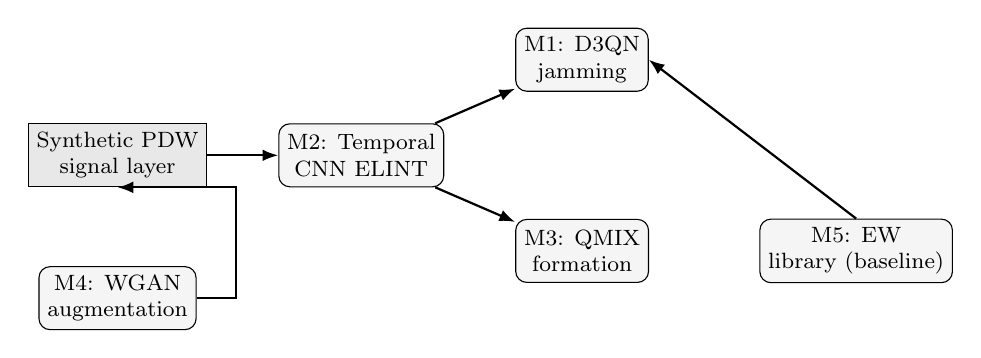
\begin{tikzpicture}[
  node distance=6mm and 9mm,
  box/.style={draw, rounded corners, align=center, font=\footnotesize,
              minimum height=8mm, inner sep=3pt, fill=gray!8},
  data/.style={draw, align=center, font=\footnotesize, minimum height=8mm,
               inner sep=3pt, fill=gray!18},
  arr/.style={-{Latex[length=2mm]}, thick}]
  \node[data] (data) {Synthetic PDW\\ signal layer};
  \node[box, right=of data] (elint) {M2: Temporal\\ CNN ELINT};
  \node[box, above right=4mm and 9mm of elint] (jam) {M1: D3QN\\ jamming};
  \node[box, below right=4mm and 9mm of elint] (marl) {M3: QMIX\\ formation};
  \node[box, below=10mm of data] (gan) {M4: WGAN\\ augmentation};
  \node[box, right=14mm of marl] (base) {M5: EW\\ library (baseline)};
  \draw[arr] (data) -- (elint);
  \draw[arr] (elint) -- (jam);
  \draw[arr] (elint) -- (marl);
  \draw[arr] (gan.east) -- ++(0.5,0) |- (data.south);
  \draw[arr] (base.north) -- (jam.east);
\end{tikzpicture}%
}
\caption{Cognitive EW architecture over a shared synthetic signal layer (component-wise
evaluation; the loop is the design, not a single end-to-end run). The signal layer feeds ELINT
classification; inferred emitter state conditions jamming and coordinated formation; the GAN
augments the data layer; the deterministic library is the conventional baseline for jamming (M1).}
\label{fig:arch}
\end{figure}

The synthetic threat catalog (\texttt{configs/temporal\_cnn\_elint/emitters.yaml}) contains
eight emitter types---SA-2, SA-6, S-300, S-400, HQ-9, an AESA radar, and two LPI emitters
(FMCW and polyphase)---each with up to four operating modes (search, track-while-scan, track,
missile guidance) and per-mode RF band, PRI pattern, pulse width, scan period, frequency-hopping
and intra-pulse modulation. Threat state is a monotone function of operating mode.

The component-wise evaluation workflow on the NTTR-inspired synthetic combat range is shown in
Fig.~\ref{fig:workflow}: the threat catalog drives PDW signal generation, split into
training and held-out evaluation; learned components (M2 ELINT, M1 jamming, M3 formation) are
trained on the training split; the GAN (M4) augments the catalog and feeds back into generation;
and held-out evaluation scores the cognitive policies against their baselines (M1 vs.\ the M5
conventional library, M3 vs.\ a learned IQL controller), yielding the win-rate, suppression and
robustness anchors.

\begin{figure*}[t]
\centering
\resizebox{\textwidth}{!}{%
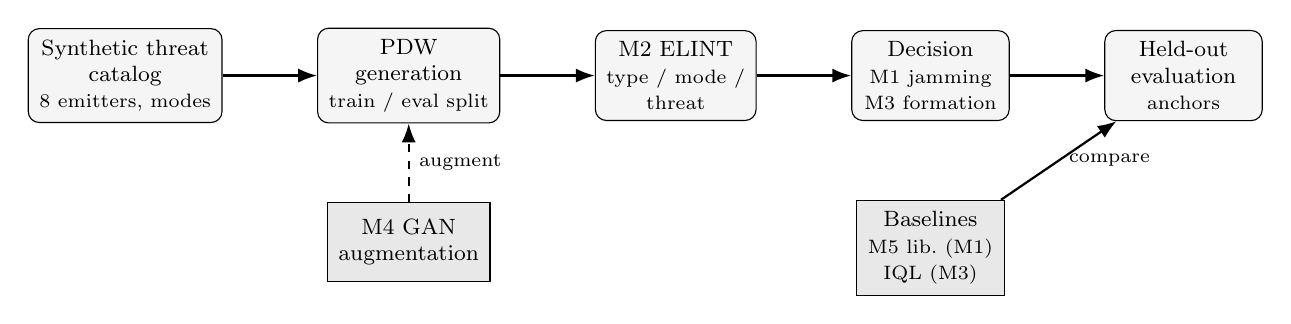
\begin{tikzpicture}[
  node distance=7mm and 12mm,
  stage/.style={draw, rounded corners, align=center, font=\footnotesize,
                minimum height=11mm, minimum width=20mm, inner sep=4pt, fill=gray!8},
  aux/.style={draw, align=center, font=\footnotesize, minimum height=10mm,
              inner sep=4pt, fill=gray!18},
  arr/.style={-{Latex[length=2.4mm]}, thick},
  fb/.style={-{Latex[length=2.4mm]}, thick, dashed}]
  \node[stage] (cat) {Synthetic threat\\ catalog\\ {\scriptsize 8 emitters, modes}};
  \node[stage, right=of cat] (gen) {PDW\\ generation\\ {\scriptsize train / eval split}};
  \node[stage, right=of gen] (elint) {M2 ELINT\\ {\scriptsize type / mode /}\\ {\scriptsize threat}};
  \node[stage, right=of elint] (dec) {Decision\\ {\scriptsize M1 jamming}\\ {\scriptsize M3 formation}};
  \node[stage, right=of dec] (out) {Held-out\\ evaluation\\ {\scriptsize anchors}};
  \node[aux, below=10mm of gen] (gan) {M4 GAN\\ augmentation};
  \node[aux, below=10mm of dec] (base) {Baselines\\ {\scriptsize M5 lib.\ (M1)}\\ {\scriptsize IQL (M3)}};
  \draw[arr] (cat) -- (gen);
  \draw[arr] (gen) -- (elint);
  \draw[arr] (elint) -- (dec);
  \draw[arr] (dec) -- (out);
  \draw[fb] (gan) -- (gen) node[midway, right, font=\scriptsize] {augment};
  \draw[arr] (base) -- (out) node[midway, right, font=\scriptsize] {compare};
\end{tikzpicture}%
}
\caption{Component-wise evaluation workflow on the NTTR-inspired synthetic electronic combat range.
The synthetic threat catalog drives PDW generation (split into training and held-out
evaluation); learned components are trained on the training split; the GAN augments generation
(dashed feedback); and held-out evaluation scores each cognitive policy against its baseline
(M1 vs.\ the M5 conventional library, M3 vs.\ a learned IQL controller) to produce the reported
anchors.}
\label{fig:workflow}
\end{figure*}

\section{Methods}
\label{sec:methods}

\subsection{M1: Adaptive jamming (D3QN)}
The radar cycle is simulated as a partially observable environment: the agent observes a length
$K{=}8$ history of emitter descriptors (frequency, PRI, waveform, scan pattern, ECCM mode) over
a horizon of $64$ steps and chooses a jamming technique (noise, DRFM repeater, deception,
cross-eye, velocity/range gate pull-off, chaff, decoy, evasive, or none) at one of four power
levels. A Dueling Double DQN~\cite{wang2016dueling,vanhasselt2016double} with hidden width $128$
estimates $Q(s,a)=V(s)+\big(A(s,a)-\tfrac{1}{|\mathcal{A}|}\sum_{a'}A(s,a')\big)$. The reward
combines technique effectiveness against the current mode with a power-consumption penalty
($\lambda_P{=}0.5$), and a win/lose terminal bonus. Training uses $\gamma{=}0.99$, learning
rate $10^{-3}$, replay buffer $5 \times 10^{4}$, batch $64$, target sync every $500$ steps and
$\varepsilon$-greedy annealed $1.0 \to 0.05$ over $5000$ steps, for $2 \times 10^{4}$
environment steps.

\subsection{M2: ELINT classification (temporal CNN)}
A dilated, depthwise-separable temporal CNN ingests a multi-channel PDW window
($\texttt{seq\_len}{=}64$) and produces three logits via explicit type, mode and threat heads
over a shared trunk (stem $\to$ residual dilated blocks with dilations $\{1,2,4\}$ $\to$
global average pool $\to$ shared MLP $\to$ three linear heads). We caution that, in the current
catalog, the \emph{threat state} label is a deterministic monotone function of the operating
mode; consequently the threat head largely mirrors the mode head (their confusion matrices are
identical in our runs) and the threat accuracy is \emph{not} independent evidence---we report it
for completeness only. A threat state that depended on additional context (tracking history,
engagement phase, intermittent emission) would make this an independent task; we leave that to
future work. The model is evaluated with a composite score: the worst of the macro type/mode/LPI
accuracies must clear the target \emph{and} the measured $p99$ latency must satisfy $<1$\,ms;
otherwise the composite target does not pass.

\subsection{M3: Coordinated formation (QMIX vs.\ IQL)}
Four aircraft form a Dec-POMDP under CTDE. Each agent is a GRU recurrent $Q$-network
(\texttt{AgentRNN}) selecting a parameterized action (target $\times$ jamming type $\times$ power
level). The coordinated controller mixes per-agent values with a QMIX hypernetwork whose
non-negative weights enforce the Individual-Global-Max property, trained with Double-$Q$ targets
and smooth-$L_1$ TD loss. The independent baseline (IQL) shares the identical agent network and
training budget but omits the mixer, isolating the effect of coordination. We report the
relative improvement in suppressed IADS fraction, $r = (S_\text{coord} - S_\text{indep}) /
S_\text{indep}$, where $S$ is the mean fraction of the IADS suppressed per episode; $r = 0.45$
denotes the $+45\%$ proposal target.

\subsection{M4: Synthetic augmentation (WGAN-GP)}
A 1D-CNN generator with a continuous type embedding produces PDW windows; a Wasserstein critic
without batch normalization is trained with gradient penalty
($\lambda{=}10$)~\cite{gulrajani2017wgangp}. A catalog sampler
interpolates emitter-type pairs to synthesize $\ge 50$ distinct types, exported to HDF5 with
provenance. Validity is checked structurally (continuous-in-range and one-hot fractions) and
distributionally (per-feature Wasserstein-1, categorical total variation, diversity). Value is
measured by a \emph{synthetic-data substitution} ablation: two emitters (the LPI-FMCW and
LPI-polyphase types) are removed from the real training set, and the M2 type head is trained
without vs.\ with \emph{synthetic} samples of exactly those two emitters; we then report type
accuracy on the held-out LPI emitters. This measures whether GAN-generated samples can stand in
for emitter classes withheld from the classifier's real training set---it is \emph{not} a
zero-shot or open-set test, since
the augmented model does see synthetic examples of the held-out classes (a genuine
uncatalogued-emitter evaluation is future work, Section~\ref{sec:discussion}).

\subsection{M5: Conventional baseline}
A deterministic threat$\to$countermeasure selector reproduces classical doctrine with an
explicit, versioned rule library. It is the conventional-doctrine reference row for the M1
comparison (M3 uses a learned IQL controller as its baseline) and requires no training.

\section{Experimental Setup}
\label{sec:setup}
All publishable numbers come from a \emph{five-seed} \emph{full}-profile campaign of the unified
anchor harness (\texttt{notebooks/run\_anchors.py --profile full --anchors all --seeds
1,3,6,8,9}) executed on Colab/GPU; a \emph{quick} CPU profile exists only to validate the
pipeline and its numbers are never used as results. Each anchor is run independently for every
seed; tables and figures report the mean $\pm$ sample standard deviation over the five seeds and
the per-seed pass rate, while the $95\%$ confidence intervals (Student's $t$) are recorded in the
released aggregate artifact. Five seeds support a first variance estimate but are insufficient
for strong significance claims; broader seed counts and significance testing are future work.
All models operate on the PDW (pulse-descriptor-word) representation in these experiments; the IQ
layer is shared infrastructure and is not consumed by M1--M4 here. Inference latency is profiled
at batch size $1$ in evaluation/inference mode with explicit CUDA synchronization, $5$ warm-up and
$50$ timed iterations, reporting the mean and the $99$th percentile. Two caveats apply: the exact
Colab GPU model is not pinned across runs, so \emph{absolute} latency values are indicative
rather than hardware-exact; and a $p99$ estimated from $50$ samples is coarse (dominated by the
observed maximum). A hardened protocol---pinned hardware, $\ge\!10^{3}$ iterations with
\texttt{torch.cuda.Event} timing, and reporting median/$p95$/$p99$/max---is future work, although
the order-of-magnitude conclusions (M1/M3 well under budget, M2 above $1$\,ms) are robust to it. The dataset
configuration is summarized in Table~\ref{tab:data}. The aggregate report and the per-seed
\texttt{metrics.json}/\texttt{run\_meta.json} are staged under version control in
\texttt{results/anchors\_full\_ms\_accepted/}, and every table and figure in this paper is
regenerated from them by the released scripts. Reproducibility metadata is summarized in
Table~\ref{tab:repro}: the seed set, a representative configuration hash, and pinned dependency
versions. No classified or operational NTTR data is used; the environment is a synthetic,
NTTR-inspired electronic combat range.

\begin{table}[t]
\caption{Synthetic dataset / scenario configuration (M2 ELINT pipeline).}
\label{tab:data}
\centering
\footnotesize
\begin{tabular}{@{}ll@{}}
\toprule
Field & Value \\
\midrule
Emitter types / modes / threat states & 8 / 4 / 4 \\
LPI emitter types & 2 (FMCW, polyphase) \\
PDW window length & 64 pulses \\
Pulses per train / trains per emitter & 512 / 96 \\
Train / val / test split & 0.70 / 0.15 / 0.15 \\
Parameter noise std & 0.015 \\
Pulse-dropout / spurious-pulse prob. & 0.01 / 0.01 \\
\bottomrule
\end{tabular}
\end{table}

\begin{table}[t]
\caption{Reproducibility metadata (five-seed full campaign).}
\label{tab:repro}
\centering
\footnotesize
\begin{tabular}{@{}ll@{}}
\toprule
Field & Value \\
\midrule
Profile & full \\
Seeds & 5 (1, 3, 6, 8, 9) \\
ELINT data config hash & \texttt{78daace0e0c348ff\ldots} \\
Python & 3.11.15 \\
PyTorch & 2.6.0+cu124 \\
NumPy & 2.4.6
\\
\bottomrule
\end{tabular}
\end{table}

\section{Results}
\label{sec:results}
The target thresholds are those stated a priori in the project proposal, themselves anchored to
values reported in the cognitive-EW literature; their provenance is given in
Table~\ref{tab:targets}. We stress these are \emph{a-priori targets}, not claims of
state-of-the-art superiority. Table~\ref{tab:anchors} then summarizes each target metric against
its threshold (mean $\pm$ std over five seeds, with the per-seed pass rate). Of the four
quantitative targets, M1, M3 and M4 pass on all five seeds. M2 is a \emph{composite} target with
an accuracy requirement and a latency requirement: it meets the accuracy requirement on every
seed but fails the latency requirement on every seed (M5 is the conventional jamming baseline for
M1 and carries no target of its own).

\begin{table}[t]
\caption{Provenance of the a-priori target thresholds.}
\label{tab:targets}
\centering
\footnotesize
\begin{tabular}{@{}llp{3.4cm}@{}}
\toprule
Target & Value & Source / rationale \\
\midrule
M1 win rate & $\ge 0.92$ & proposal; DRL-jamming results~\cite{zhao2022sac,wang2022d3qn} \\
M2 macro acc. & $\ge 0.96$ & proposal; vs.\ $<0.65$ conventional ELINT~\cite{matuszewski2021cnn} \\
M2 $p99$ latency & $<1$\,ms & proposal; vs.\ $\approx 15$\,ms baseline~\cite{matuszewski2021cnn} \\
M3 suppression & $\ge +0.45$ & proposal; cf.\ $\approx 46\%$ lock reduction~\cite{cai2025macjd} \\
M4 substitution & $\ge +0.22$ & proposal target \\
\bottomrule
\end{tabular}
\end{table}

\begin{table*}[t]
\caption{Anchor results over the five-seed campaign (mean $\pm$ std). Achieved vs.\ target vs.\
baseline, with per-seed pass rate.}
\label{tab:anchors}
\centering
\footnotesize
\begin{tabular}{@{}llccccc@{}}
\toprule
Anchor & Metric & Target & Achieved & Baseline & Rate & Pass \\
\midrule
M1 Adaptive jamming & win rate vs.\ library & 0.92 & $1.000 \pm 0.000$ & $0.733 \pm 0.038$ & 5/5 & \cmark \\
M2 ELINT (accuracy) & min.\ macro accuracy & 0.96 & $0.984 \pm 0.005$ & -- & 5/5 & \cmark \\
M2 ELINT (latency) & $p99$ latency (ms) & $<1.0$ & $2.057 \pm 0.584$ & -- & 0/5 & \xmark \\
M3 Formation MARL & rel.\ suppression impr. & 0.45 & $2.594 \pm 0.561$ & $0.284 \pm 0.050$ & 5/5 & \cmark \\
M4 GAN substitution & synthetic-substitution gain & 0.22 & $0.800 \pm 0.274$ & $0.000 \pm 0.000$ & 5/5 & \cmark
\\
\bottomrule
\end{tabular}
\end{table*}

\subsection{M1: adaptive jamming vs.\ baseline}
The D3QN agent achieves a $1.000 \pm 0.000$ spectrum win rate against the simulated radar cycle
on all five seeds, versus $0.733 \pm 0.038$ for the deterministic library---above the $0.92$
target. Inference latency is $0.232 \pm 0.087$\,ms mean / $0.534 \pm 0.411$\,ms $p99$
(Table~\ref{tab:latency}), comfortably within the $5$\,ms inference budget. The zero variance of
the win rate indicates a robust policy but also that the current radar-cycle environment is not
the binding difficulty; hardening the scenario is future work (Section~\ref{sec:discussion}). We
report measured \emph{inference} latency only; the $<4$\,ms end-to-end adaptation time to a
waveform change is a system-level target that we do not separately characterize here.
Fig.~\ref{fig:baseline} contrasts the cognitive policy with the conventional/independent
baselines for M1 and M3.

\begin{table}[t]
\caption{Measured inference latency (batch~$=1$, single GPU per run; exact Colab model not
pinned). Mean and $p99$ (ms) over $50$ timed iterations; the $p99$ estimate is correspondingly
coarse (see text).}
\label{tab:latency}
\centering
\footnotesize
\resizebox{\columnwidth}{!}{%
\begin{tabular}{@{}lcccc@{}}
\toprule
Component & Mean & $p99$ & Target & Pass \\
\midrule
M1 Adaptive jamming & $0.232 \pm 0.087$ & $0.534 \pm 0.411$ & $<5$ & \cmark \\
M2 ELINT classifier & $1.042 \pm 0.166$ & $2.057 \pm 0.584$ & $<1$ & \xmark \\
M3 Formation agent & $0.198 \pm 0.088$ & $0.372 \pm 0.153$ & -- & --
\\
\bottomrule
\end{tabular}%
}
\end{table}

\subsection{M2: ELINT classification}
Table~\ref{tab:elint} reports the metrics. Macro accuracy is $0.984 \pm 0.005$ on emitter type
and $\approx 1.000$ on mode and LPI---every accuracy target ($\ge 0.96$) is met on all five
seeds (we omit threat from this claim, as it is a deterministic function of mode; see
Section~\ref{sec:methods}). Both LPI emitters are classified perfectly on this catalog, though
they are spectrally distinct and so not a stress test of LPI recognition. The only residual type
confusion is between S-300 and HQ-9 (Fig.~\ref{fig:confusion}, summed over seeds), two modern SAM
systems with overlapping X-band track parameters. Latency is $1.042 \pm 0.166$\,ms mean /
$2.057 \pm 0.584$\,ms $p99$, above the $<1$\,ms target on every seed; the composite target is
therefore gated to fail on latency despite passing accuracy. We treat the sub-millisecond $p99$
as future work (Section~\ref{sec:discussion}).

\begin{table}[t]
\caption{M2 ELINT metrics and latency (mean $\pm$ std). Accuracy targets met; $p99$ latency not
met. Threat accuracy mirrors mode by construction (Section~\ref{sec:methods}).}
\label{tab:elint}
\centering
\footnotesize
\begin{tabular}{@{}lccc@{}}
\toprule
Metric & Value & Target & Pass \\
\midrule
Emitter type (macro) & $0.9837 \pm 0.0049$ & $\ge 0.96$ & \cmark \\
Operating mode (macro) & $0.9998 \pm 0.0003$ & $\ge 0.96$ & \cmark \\
Threat state (macro) & $0.9998 \pm 0.0003$ & $\ge 0.96$ & \cmark \\
LPI accuracy & $1.0000 \pm 0.0000$ & $\ge 0.96$ & \cmark \\
Latency mean (ms) & $1.042 \pm 0.166$ & $<1.0$ & \xmark \\
Latency $p99$ (ms) & $2.057 \pm 0.584$ & $<1.0$ & \xmark
\\
\bottomrule
\end{tabular}
\end{table}

\begin{figure}[t]
\centering
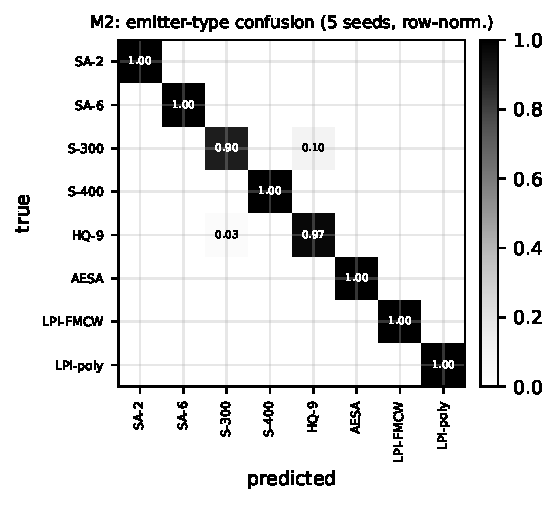
\includegraphics[width=0.85\columnwidth]{m2_confusion_type.pdf}
\caption{M2 emitter-type confusion matrix, summed over the five seeds and row-normalized.
Off-diagonal mass is confined to the S-300/HQ-9 pair; both LPI emitters are perfectly separated.}
\label{fig:confusion}
\end{figure}

\subsection{M3: coordinated vs.\ independent formation}
The QMIX controller suppresses the IADS far more effectively than the independent IQL baseline,
which reaches a suppressed fraction of $0.284 \pm 0.050$ under the same comparison evaluation
(both controllers are scored from their best-validation checkpoints in one shared harness, so the
gap reflects coordination, not checkpoint selection).
The resulting relative improvement is $r = 2.594 \pm 0.561$, far above the $0.45$ target on all
five seeds (i.e.\ a $+259\%$ relative gain in suppressed fraction), with a formation-agent
inference latency of $0.372 \pm 0.153$\,ms $p99$.
Coordination---joint target assignment and power management that avoids electronic
fratricide---is the decisive factor, since the two regimes share the identical agent network and
training budget.

\begin{figure}[t]
\centering
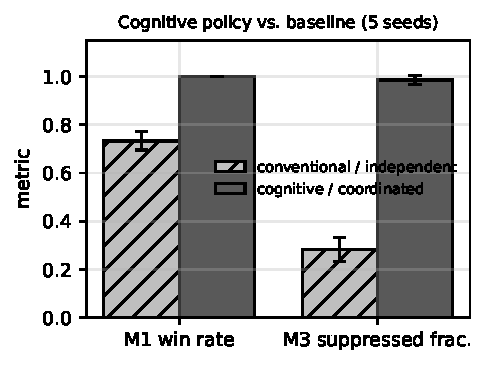
\includegraphics[width=0.85\columnwidth]{baseline_comparison.pdf}
\caption{Cognitive/coordinated policy vs.\ conventional/independent baseline. The two panels show
\emph{different} metrics that both lie in $[0,1]$---M1 spectrum win rate and M3 suppressed IADS
fraction---and are not directly comparable across panels; each is read against its own baseline.}
\label{fig:baseline}
\end{figure}

\subsection{M4: synthetic-data substitution}
The generator exports $230{,}000$ synthetic windows per seed spanning the $8$ base emitter types
plus $84$ interpolated synthetic \emph{variants} of base-type pairs ($92$ in total; the M2 type
head still classifies only the $8$ real classes), with fully valid structure (continuous-in-range and one-hot fractions $=1.0$, coverage
$=1.0$) and small distributional gaps (mean per-feature Wasserstein-1 $\approx 0.04$); see
Table~\ref{tab:gan}. In the substitution ablation (two LPI emitters removed from the real
training set), the baseline classifier scores $0.000$ on those emitters---a closed-set model
cannot label classes absent from its real training set---while training on \emph{synthetic}
samples of exactly those
two emitters lifts their accuracy to $0.800 \pm 0.274$, and global test accuracy rises from
$0.657 \pm 0.020$ to $0.832 \pm 0.056$ (Fig.~\ref{fig:gan}). The substitution gain of $0.800$
exceeds the $0.22$ target on all five seeds; the spread reflects the coarse two-class held-out
set (three seeds recover both LPI types, two recover one). The $0.0$ baseline is a structural
consequence of the closed-set setup, so we report the absolute gain rather than an undefined
ratio; the result shows synthetic data can substitute for missing real samples, not that the
classifier generalizes zero-shot to uncatalogued emitters.

\begin{table}[t]
\caption{M4 synthetic validity, volume and downstream robustness (mean $\pm$ std over five
seeds).}
\label{tab:gan}
\centering
\footnotesize
\begin{tabular}{@{}lcc@{}}
\toprule
Quantity & Value & Target/Ideal \\
\midrule
Synthetic windows exported & 230,000 & $>200{,}000$ \\
Synthetic variants (8 base + interp.) & 92 & $\ge 50$ \\
Continuous-in-range fraction & $1.000 \pm 0.000$ & 1.0 \\
One-hot categorical fraction & $1.000 \pm 0.000$ & 1.0 \\
Catalog coverage & $1.000 \pm 0.000$ & 1.0 \\
Mean Wasserstein-1 / feature & $0.0378 \pm 0.0168$ & lower better \\
Held-out acc.\ (baseline) & $0.000 \pm 0.000$ & -- \\
Held-out acc.\ (augmented) & $0.800 \pm 0.274$ & -- \\
Global acc.\ (baseline) & $0.657 \pm 0.020$ & -- \\
Global acc.\ (augmented) & $0.832 \pm 0.056$ & --
\\
\bottomrule
\end{tabular}
\end{table}

\begin{figure}[t]
\centering
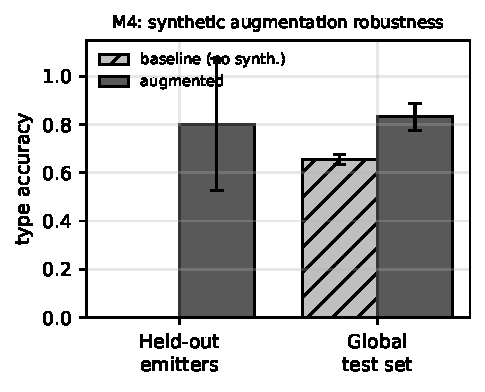
\includegraphics[width=0.85\columnwidth]{gan_robustness.pdf}
\caption{M4 synthetic-data substitution: emitter-type accuracy with and without synthetic
samples of the two removed LPI emitters, on those held-out emitters and on the global test set.
Bars: mean over five seeds; error bars: std.}
\label{fig:gan}
\end{figure}

\section{Discussion}
\label{sec:discussion}
\textbf{A shared signal layer, not a closed-loop demonstration, is the contribution.} Each
component is individually competitive; the contribution here is that all five are defined over one
synthetic signal layer and one evaluation harness, so ELINT, jamming, coordination and GAN
augmentation are expressed in a common representation and can be compared on equal footing. The
architecture wires these into a sense--decide--act loop (Fig.~\ref{fig:arch}), but we evaluate
each component independently and do \emph{not} claim a single end-to-end closed-loop result;
running the wired loop end-to-end---with ELINT state actually driving M1/M3 online and the GAN
retraining M2 in the loop---is future work.

\textbf{Why M2 accuracy holds up while $p99$ latency is future work.} The classifier meets every
accuracy target on every seed, including the two LPI emitters---though we note these are
spectrally distinct (FMCW at $9$--$10$\,GHz vs.\ polyphase at $14$--$16$\,GHz), so their perfect
separation reflects this catalog rather than a solved LPI problem; low-SNR, spectrally-overlapping
LPI is future work. Its $p99$ latency of $2.06 \pm 0.58$\,ms is above the $<1$\,ms target on all
five seeds, so the composite target does not pass. We deliberately
keep these decoupled: accuracy and latency should be interpreted separately, and the latency gap is concrete
engineering. The dilated temporal convolution dominates the budget, and three complementary
levers target sub-millisecond inference. (i) \emph{Structured channel pruning} narrows the
convolution uniformly, retaining dense-accelerator compatibility without sparse-kernel libraries.
(ii) \emph{Post-training INT8 quantization} is the cheapest option, but the sensitivity of PDW
parameters---and the narrow margins on LPI signatures in particular---may demand
\emph{quantization-aware training} to preserve accuracy. (iii) \emph{Knowledge distillation} from
the present dilated TCN (teacher) into a lighter MobileNet-style 1D-CNN student can cross the
$1$\,ms barrier while retaining the teacher's accuracy. A full ablation of these is future work.
Notably, the remaining components already meet sub-millisecond or few-millisecond $p99$ latencies
(Table~\ref{tab:latency}), so documented latency---rarely reported in this field---is itself a
result.

\textbf{What the synthetic-data result does and does not show.} The $0.0\!\to\!0.800$ jump is
large by construction: a closed-set classifier scores zero on the two LPI emitters absent from its
real training set,
so the headline is governed by that structural zero rather than by a hard learning problem. The
more conservative global accuracy ($0.657\!\to\!0.832$) is the stronger evidence that the GAN
samples carry usable class information. The experiment therefore demonstrates
\emph{synthetic-data substitution}---that generated samples can stand in for missing real samples
of a known emitter type---and \emph{not} zero-shot or open-set generalization to genuinely
uncatalogued emitters. The interpolated synthetic types are likewise not claimed to be physically
realizable radars; their structural and distributional validity (Table~\ref{tab:gan}) only bounds
how far they drift from the real catalog. Leave-one-family-out, open-set rejection and few-shot
real-sample adaptation are the experiments that would establish true uncatalogued-emitter
robustness (future work).

\textbf{Threats to validity.} The environment is a synthetic, NTTR-inspired electronic combat
range built from published/synthetic catalogs, not a recreation of operational NTTR fidelity and
not validated on real or classified waveforms; in particular it omits multipath propagation
losses, realistic antenna patterns and radar clutter, and uses 2D geometry with idealized
observability, as in comparable prior work~\cite{cai2025macjd}. We argue the PDW-level
abstraction nonetheless remains valid because the PDW parameters (PRI, pulse width, RF, scan
period) are exactly the post-detection features an RWR/ELINT receiver consumes; multipath,
antenna-pattern and clutter effects manifest principally as measurement noise and intermittent
pulse loss on those parameters, which the dataset emulates through additive parameter noise,
random pulse dropout and spurious pulses. Higher RF-level fidelity would refine that noise model
but would not change the decision-level features the models operate on. The train/val/test split is performed at the (non-overlapping) PDW-window level rather than by
pulse train or emitter instance, so distinct windows of the same pulse-train realization can fall
in different splits; this may bias the near-$1.0$ accuracies optimistically, and a stricter
by-train split is future work. Relatedly, the PDW feature layer includes \emph{engineered hint
features} (e.g.\ an LPI indicator, a frequency-hopping indicator, pulse-progression and rolling
parameter statistics) that encode domain priors directly; these almost certainly contribute to
the near-perfect LPI/mode accuracies, so part of that performance reflects feature design and
catalog separability rather than purely learned generalization, and an ablation that removes the
hint features is needed to isolate the network's own contribution (future work). Results come
from a five-seed campaign; broader seed counts would tighten the intervals further. Finally, the M1 win
rate saturates at $1.0$ across all seeds, indicating the radar-cycle environment is not the
binding difficulty; future work must give the threat radar \emph{reactive, adaptive ECCM}
(dynamic waveform/PRI agility that responds to the jammer) so that the scenario poses a binding
difficulty and genuinely stresses the agent's resilience.

\textbf{Dual-use considerations.} This work describes learning methods for electronic attack and
electronic protection, which are inherently dual-use. We mitigate disclosure risk by using only
synthetic emitters and signals derived from published/synthetic catalogs---no classified
parameters, real threat libraries or operational data are used or released---and by evaluating in
an abstract, NTTR-\emph{inspired} simulator rather than an operationally faithful one. The
released artifacts are simulation results and code, not deployable EW capability. We encourage
responsible use consistent with applicable export-control and research-ethics norms.

\section{Conclusion}
We presented a cognitive EW component suite---adaptive jamming, ELINT classification,
coordinated formation, generative augmentation and a deterministic baseline library---integrated over a
shared synthetic signal layer and evaluated component-wise on an NTTR-inspired synthetic
electronic combat range with reproducible artifacts. Across a five-seed
campaign, three of the four quantitative anchors pass on every seed---a $1.000 \pm 0.000$ jamming
win rate at $0.53$\,ms $p99$, a $+259\%$ ($2.594 \pm 0.561$) coordinated suppression improvement,
and a $0.000\!\to\!0.800$ synthetic-data substitution gain for two held-out LPI emitters---while
the ELINT classifier (M2) meets every accuracy target ($0.984 \pm 0.005$ type, $\approx 1.000$
mode and LPI) on every seed but not its $<1$\,ms $p99$ latency target ($2.06 \pm 0.58$\,ms). We
frame these as synthetic-environment results; their external validity is bounded by the
simulator's fidelity and by the strength of the baselines. Future work targets sub-millisecond
ELINT inference (structured pruning, INT8 QAT, knowledge distillation), a harder radar-cycle
environment with reactive ECCM, stronger learning baselines and ablations, leave-one-family-out
and open-set evaluation, broader seed counts with significance testing, and a richer synthetic
threat catalog.

\section*{Reproducibility}
The accepted per-seed and aggregate JSON artifacts, the full configuration hashes and seeds, and
the deterministic table/figure generation scripts (\texttt{scripts/paper/}) are released in the
project repository; a permanent URL and an archival DOI (Zenodo) will accompany the camera-ready
version, and the artifact bundle is available to reviewers on request. All numbers above are
regenerated from \texttt{results/anchors\_full\_ms\_accepted/}. Configuration hashes are
abbreviated in Table~\ref{tab:repro} for space; the complete hashes accompany each
\texttt{run\_meta.json}.

\bibliographystyle{IEEEtran}
\bibliography{refs}

\end{document}
